\chapter{Grundlagen} \label{CapterFundamentals}

Dieses Kapitel gibt ein Überblick über die in dieser Arbeit verwendete Terminologien und führt in Grundlagen zu Technologien und Techniken ein welche die Basis für dieser Arbeit bilden. 

Nachdem die Definition von Augumented Reality erläutert wurde, werden unterschiedliche Ansätze für die Objekterkennung und Verfolgung vorgestellt.  
Diese sind ein essenzieller Bestandteil der Augumented Reality Technologie. Es wird die die Definition von Situated Visualization erläutert und Visualisierungstechniken für die Darstellung von Daten im Kontext zur physischen Welt (z. Bsp. Gegenstände, Person, Aufgabe) nahe gebracht. Abschließend wird die Definition von Usability erläutert und ein Einblick in Usablity Engineering gegeben, welches eine etablierte Vorgehensweise für die Gestaltung und Entwicklung von Systemen mit hohen Usability Anforderungen ist. 

\section{Augmented Reality}

%Definition und Begriffseingrenzung  von AR
Augmented Reality (zu dt. Erweiterte Realität, kurz AR) steht für die Überlagerung der realen Welt mit digitalen Informationen. \cite{Azuma.1997,DieterSchmalstieg2016} Im Gegensatz zu virtuellen Realität wo Benutzer vollständig in virtuelle Umgebungen eintauchen,
ist das Ziel von AR, Informationen direkt in die physische Umgebung des Benutzers einzufügen. So soll der Eindruck entstehen, dass diese Informationen Teil der realen Welt sind. \footnote{ Laut Definition von Azuma  müssen Informationen hierbei nicht nur auf visuelle Informationen beschränkt sein, 
sondern können auch auditive, haptische, gustative (Geschmack) oder auch olfaktorische (Geruch) Informationen beinhalten.} \cite{Azuma.1997} Während in VR, Benutzer von der äußeren Umgebung nichts mitbekommen, wird in AR die reale Umgebung des Benutzers, mit virtuellen 
Objekten überlagert. Azuma beschreibt in \cite{Azuma.1997}, folgende Charakteristiken für Augmented Reality: 

\begin{enumerate}
	\item Kombinieren reale und virtuelle Welt (Combines real and virtual).
	\item Ermöglichen Interaktionen in Echtzeit. (Interactive in real time)
	\item Informationen (reale und virtuelle) haben einen Bezug im dreidimensionalen Raum. (Registered in 3-D)
\end{enumerate}

Diese Charakteristiken helfen dabei den Augmented Reality besser einzugrenzen. \cite{Azuma.1997} Filme wie z. Bsp. ``Jurassic Park``, in welchen virtuelle Objekte in die reale Szene eingefügt werden, 
erwecken zwar den Eindruck dass diese Objekte, Teil der realen Szene sind, jedoch kann mit diesen Objekten nicht in Echtzeit interagiert werden. \cite{Tonnis2010} In Filmen werden die virtuellen Objekte in eine zuvor aufgezeichnete Aufnahme eingefügt. 
Im Gegensatz werden diese, in AR in ein live Video eingefügt. Dies bedeutet dass in  Filmen für das Einfügen von digitalen Informationen in die reale Szene eine viel größere Zeit zur Verfügung steht. 
In AR muss dies in wenigen Millisekunden geschehen. Die neue Position und Ausrichtung des virtuellen Objektes in live Szene muss in der Zeit zwischen zwei Frames bestimmt werden.

Ein anderes Beispiel im Live Ansicht von Digitalkameras zu finden, welche das aufzunehmende Bild als Vorschau anzeigen. Oft blenden Digitalkameras Informationen zu den aktuellen Einstellungen der Kamera sowie den Ladezustand der Batterie im Vorschaubild ein (Siehe Abbildung \ref{img:ar_camera_example}).  
Diese Informationen überlagern zwar die reale Szene, haben jedoch keinen Bezug zum dreidimensionalen Raum. Der elektronische Sucher hingegen welches Objekte (z. Bsp. Gesichter) erkennt und in einem virtuellen Rahmen einrahmt, hat ein Bezug zu den Objekten im 3D Raum. Zudem sind Interaktionen in Echtzeit möglich. Bewegt sich das vom virtuellen Rahmen, eingerahmte reale Objekt, oder die Kamera selbst, verändert sich auch die Position des virtuellen Objektes. 

\begin{figure}[H]
	\centering
	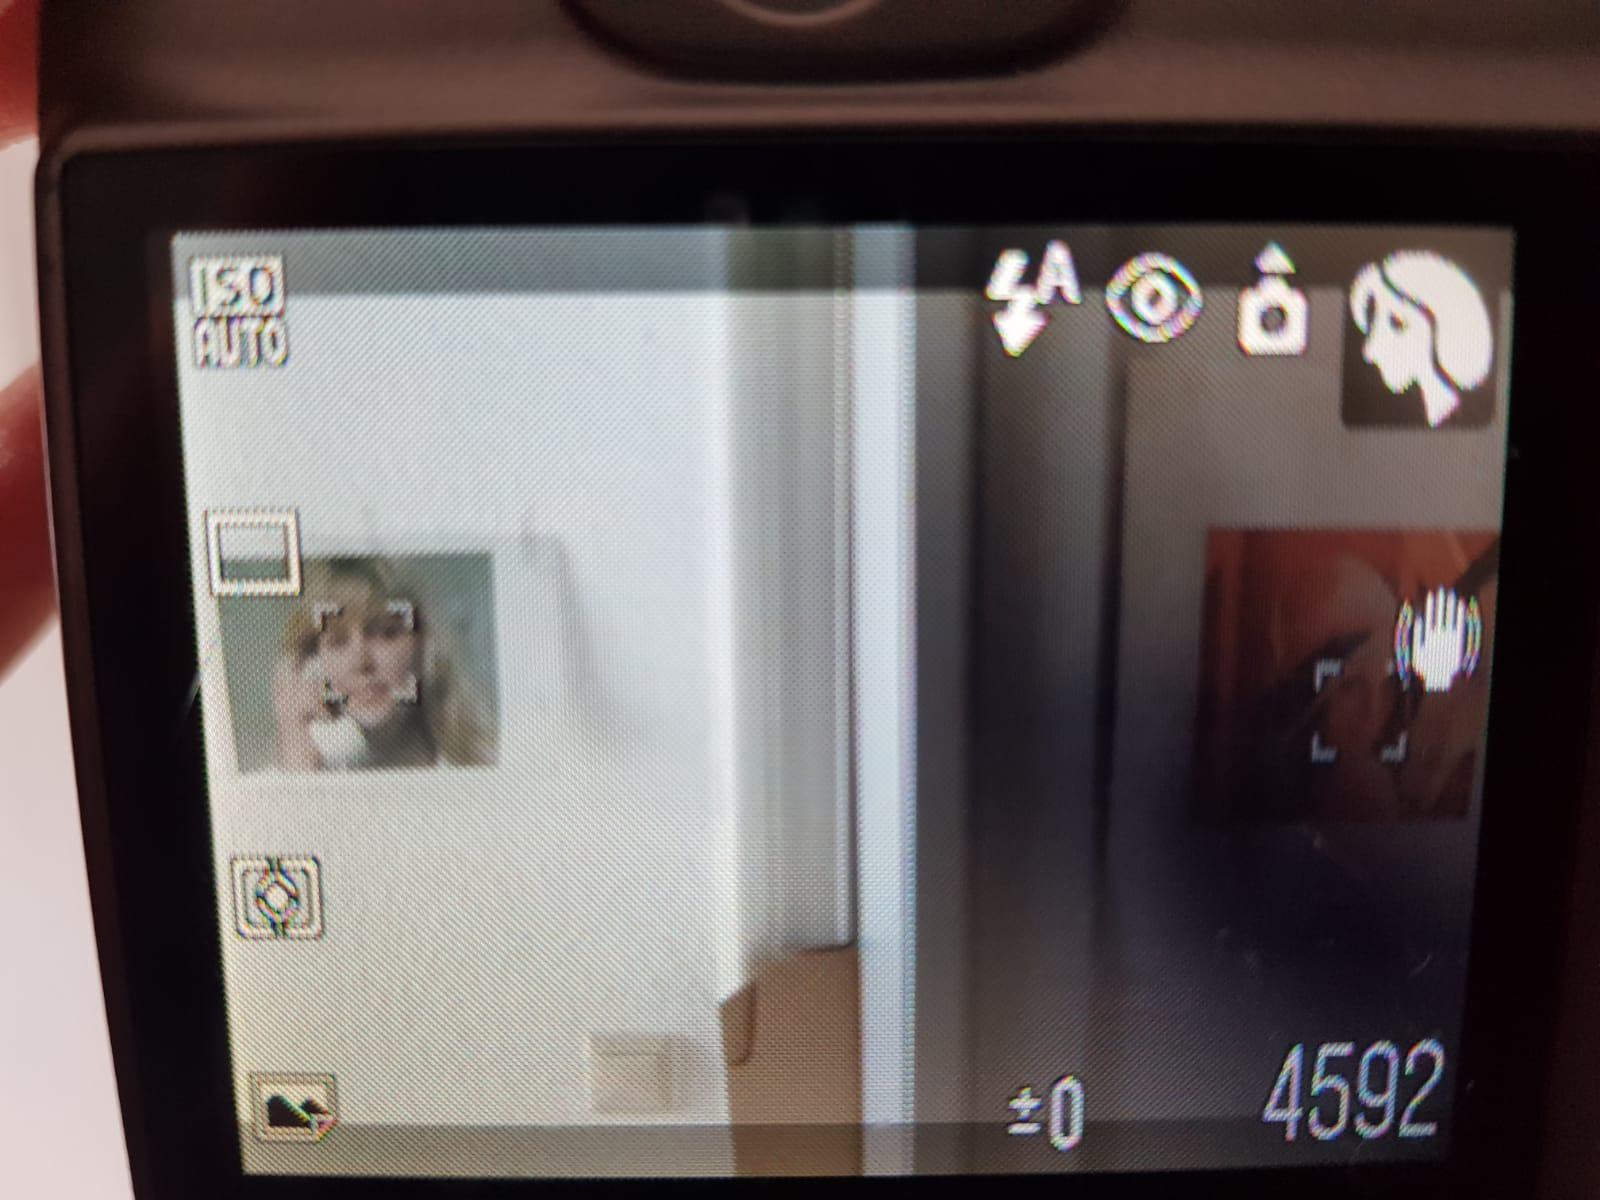
\includegraphics[width=0.45\textwidth]{resources/fundamentals/example_camera_screen_ar}
	\caption{Beispiel an Digitalkamera. Kameraeinstellungen überlagern zwar die Realität, haben jedoch keinen Bezug im dreidimensionalen Raum. Der elektronische Sucher hingegen hat ein Bezug im dreidimensionalen Raum und ist interaktiv \cite{Beispiel Dititalkamera}}
	\label{img:ar_camera_example}
\end{figure}

% Motivation
\cite{Azuma.1997} Durch das kombinieren von virtueller und physischer Welt, erweitert Augumented Reality die Wahrnehmung des Menschen. Die Motivation von AR ist, dem Menschen durch das Einfügen
von digitalen Informationen in die physische Welt, Hinweise zu geben und Details zu zeigen die sonst nicht unmittelbar wahrnehmen könnte. Diese Informationen sollen den Menschen 
bei der Verrichtung ihrer Aufgaben in der physischen Welt unterstützen.

% Anwendungsfelder von AR % Besonders passend für diese Arbeit sind Annotationen und Warung und Reperatur. Da diese sich besonders mit Interaktionen an Realen Objekten, meist Produkte befassen.
Azuma fasst in \cite{Azuma.1997}, Forschungen zu AR in sechs Anwendungsgebiete zusammen. Zur Visualisierung von Medizindaten, in der Wartung 
und Instandsetzung, Annotationen, für die Wegfindung in Robotik und für die Navigation von Militärflugzeugen. Beispielsweise können Annotationen 
verwendet werden um Informationen über den Inhalt von Regalen einzublenden während ein Nutzer durch ein Bibliothek läuft und nach bestimmten Büchern sucht. % Füge hier vielleicht noch ein Beispiel dazu ein % Füge hier Verweis auf ein Artike als Fußnotel hinzu
Auch können Annotationen in AR verwendet werden um einzelne Bauelemente an komplexen Bauteilteilen zu identifizieren und Informationen über diese zu visualisieren. 
In der Wartung und Instandsetzung können Augemented Reality Anwendungen dabei helfen Instruktionen an komplexen Maschinen und Anlagen zu visualisieren welche sonst in 
Form von Text und Bildern vorliegen. So können virtuelle Replikate über die physischen Modelle gelegt, und zum Beispiel Schritt für Schritt Anleitungen direkt am physischen Produkt visualisiert werden. 
Durch Animationen können diese Anleitungen präziser gestaltet werden und zum Beispiel auch Informationen über die Richtung geben. 

Diese Systeme können heute zum Beispiel Unterunternehmen dabei helfen besser mit ihren Kunden zu kooperieren. In Kombination mit der Technologie Internet of Things (IOT) können Unternehmen,
zustands-bezogene Informationen zu Ihren Systemen bei Endkunden abrufen und proaktiv Ihre Kunden auf notwendige Wartungen am physischen System, aufmerksam machen. Wartungsanleitungen können dann direkt 
an den Analgen angezeigt werden sodass Endkunden diese selbständig durchführen können.\footnote{https://www.ptc.com/-/media/Files/PDFs/Case-Studies/Howden-vuforia-studio-case-study-Feb-2019.pdf?la=en\&hash=6342841E1B6470C1F313295427398606 [letzter Zugriff: 25.06.2019]}

%Grundlegende Techniken
\cite[S.~32]{Tonnis2010} Für die Überlagerung der realen Welt mit virtuellen Objekten eignen sich aktuell zwei Display Techniken, Optical See-Through und Video See-Through. 
Bei Optical See-Through kann der Nutzer direkt in die reale Welt blicken und Computer generierte Bilder werden auf ein halbdurchlässiges Spiegel eingeblendet (dieses wird als Combiner bezeichnet).
Diese Technik hat den Vorteil dass der Nutzer einen direkten Blick auf die reale Welt hat. Der Nachteil ist jedoch dass die reale Welt nicht zeitgleich mit virtuellen Objekten überlagert werden kann. 
Dadurch dass die Berechnung der Positionsbestimmung und das Rendern der virtuellen Objekte Zeit in Anspruch nimmt, werden diese mit einer kleinen Verzögerung angezeigt. Dies kann auch 
wenn es sich nur um einige Millisekunden handelt zu einem so genannten Schwimmeffekt führen (en. Lag). Mit der See Through Display Technik, wird die reale Welt dem Nutzer als ein Video 
angezeigt und mit virtuellen Objekten überlagert. Der Vorteil dieser Technik liegt darin, dass die Darstellung der realen Welt um die Zeit verzögert werden kann die benötigt wird um die virtuellen Objekte 
richtig zu positionieren und rendern. Dadurch werden die Nachteile der Optical-See-Through Technik kompensiert. Dass die reale Welt dem Nutzer verzögert angezeigt wird bringt jedoch den Nachteil, 
dass Positionsänderungen von physischen im realen Welt befindenden Objekten oder die Änderung der Perspektive falls sich der Nutzer selbst bewegt, verzögert angezeigt werden. Zudem wird mit 
dieser Technik je nach Auflösung der Kamera die reale Welt mit verringerter Qualität angezeigt. \cite[S.~368]{DieterSchmalstieg2016} Vor allem während der Kommunikation mit anderen Personen können diese 
Nachteile zu Problemen führen. 

\section{Objekterkennung und- Verfolgung}


% Definition von Objekterkennung und Verfolgung

% Geschichte und Entwicklung

\subsection{Markerbasiertes Tracking}

% Begriffserklärung von Marker Trakting

% Anwendungsfelder von Marker Traking

\subsection{Markerloses Tracking}

% Begriffserklärung von Markerlosen Traking 

% Anwendungsfelder von Markerlosen Traking




\section{Situated Visualization}
\subsection{(Situated Visualization) - Definition}

Das zu konzipierende System soll durch den Einsatz von Augmented Reality, Kundenrückmeldungen zum Design von Produkten ermöglichen. Es sollen so Daten im Kontext zum Produkt eingegeben und erhoben, exploriert werden können. Als eine besondere Form von Visualisierung beschäftigt sich das Feld Situated Visualization mit der Visualisierung von Daten im Kontext zu physischen Objekten. In diesem Abschnitt Situated Visualization
näher erläutert.

\cite[S.~239]{DieterSchmalstieg2016} Ein großer Vorteil von Augmented Nutzeroberflächen ist, dessen Fähigkeit, Situation, Aufgaben oder Nutzer-relevante Informationen anzeigen zu können. 
Diesen Vorteil zunutze zu machen ist jedoch sehr davon abhängig welche Informationen in AR, in welcher Form präsentiert werden. Das Forschungsfeld Situated Visualization befasst mit der richtigen Interaktion und Präsentation von computergenerierten Grafiken in der realen Szene mit physischen Gegenständen oder Personen. \cite[S.~188]{ElSayedNevenA.M.BruceH.ThomasRossT.Smith2015} Situated Visualization ist die Präsentation von Daten welche in Bezug zur physischen Umgebung stehen. Die Bedeutungsbestimmung wird durch die Kombination von Visualisierung und dessen Beziehung zu der unmittelbaren Umgebung erreicht. \cite[S.~240]{DieterSchmalstieg2016} Abzugrenzen von Situated Visualization, sind Visualisierungen welche zwar im 3D Raum präsentiert werden, jedoch keinen Bezug zu einer im dreidimensionalen Raum befindlichen Objekt, Person oder Aufgabe haben.

\cite[S.~192]{ElSayedNevenA.M.BruceH.ThomasRossT.Smith2015} \cite[S.~2]{WesleyWillettYvonneJansen} stellen die im Abbildung \ref{img:situated_visualization_concept} dargestellte konzeptionelle Model zur Situated Visualization vor.

\begin{figure}[H]
	\centering
	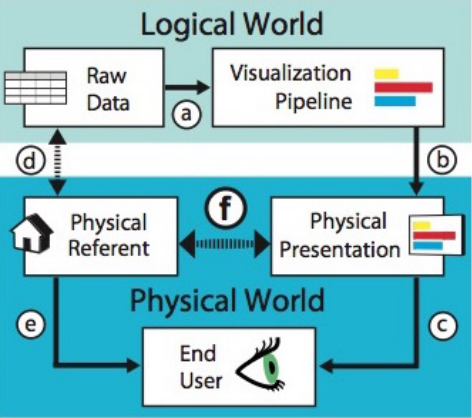
\includegraphics[width=0.5\textwidth]{resources/fundamentals/situated_visualization/spacially_situated_visualization_model.png}
	\caption{Konzeptionelles Model zu "Spatially-Situated Visualization" \cite{example_situated_visualization_concept}}
	\label{img:situated_visualization_concept}
\end{figure}

% spacially situated visualization
Dieses Model (siehe Abbildung \ref{img:situated_visualization_concept}) erweitert die konventionelle Visualisierung logische Welt (Abbildung \ref{img:situated_visualization_concept} oben) mit der physischen (realen) Welt (Abbildung \ref{img:situated_visualization_concept} unten). 
Die durchgängig dargestellten Pfeile zeigen den Informationsfluss zwischen den einzelnen Komponenten und die gestichelten Peile (Abbildung \ref{img:situated_visualization_concept} (d) und (f)) konzeptionelle Beziehungen. Der Informationsfluss beginnt bei den Rohdaten in der oberen linken Ecke der Darstellung. Die Rohdaten durchlaufen den Visualisierungs-Pipeline und werden in ein vom Menschen besser interpretierbare visuelle Form umgewandelt (Abbildung \ref{img:situated_visualization_concept} (a -> b)). Die Visualisierungs-Pipeline wird weiter unten genauer vorgestellt. 
Die Beziehung zwischen logischer und physischer Welt wird mit zwei Beziehungen hergestellt (b und d).  Die physische Präsentation der Daten (Abbildung \ref{img:situated_visualization_concept} (b)) stellt die Präsentation der Daten in visueller Form in der Realen Welt dar. 
Zum Beispiel könnte dies eine Auflistung, ein Diagramm oder ähnliches sein. Die zweite Beziehung ist die zwischen den Rohdaten und den physischen Referenten. Diese Beziehung ist konzeptionell da Datensätze sich auf mehrere unterschiedliche Referenten beziehen können. Manche Referenten produzieren selbst Daten (z. Bsp. mit Sensoren), dies ist jedoch nicht immer der Fall.Der Grad in wieweit der physische Referent und die physische Präsentation gleichzeitig wahrgenommen werden können hängt von der räumlichen Abstand zwischen diesen beiden ab. Ein Kaufinteressent könnte sich zum Beispiel Informationen zu einem Haus, Zuhause auf seinem Laptop ansehen und hätte keine Möglichkeit die Informationen zu dem Haus und das Haus selbst zur gleichen Zeit zu sehen. Er könnte aber auch vor dem Haus stehen und sich die Informationen zu dem Haus auf dem Bildschirm seines Smartphones anschauen. Oder die Informationen zu dem Haus könnten auf einem Schild, auf dem Haus platziert sein. Je näher die physische Präsentation und der physische Referent räumlich zusammen sind, desto stärker ist der Grad, der räumlichen "Situated"-sein. 

%Physically- vs. Perceptually-Situated Visualizations 
\cite[S.~194]{ElSayedNevenA.M.BruceH.ThomasRossT.Smith2015} da Distanzen jedoch relativ zu Größe von Objekten wahrgenommen werden, kann die physische und die wahrgenommene Distanz zwischen dem Physischen Referenten und der Physischen Präsentation stark voneinander abweichen. Wen beide Objekte zum Beispiel nur wenige cm groß sind, kann ein Abstand von einem Meter sehr groß erscheinen, während der gleich Abstand für sehr großes Objekt sehr wie  ein Berg in einer Landschaftsansicht zum Beispiel sehr klein erscheint. 

%Zeitlich distanz (temporal)
\cite{WesleyWillettYvonneJansen} neben der räumlichen Distanz kann auch die zeitliche Distanz zwischen dem Physischen Referenten und der physischen Präsentation betrachtet werden. 
Die zeitliche Distanz ist die zeitliche Abweichung zwischen den Daten die dem aktuellen Zustand am physischen Referenten entspricht, und den Daten welche in der Physischen Präsentation visualisiert werden.
Betrachtet man zum Beispiel Temperaturwerte die ein Temperatursensor an einem physischen Objekt anzeigt und es wird der aktuell gemessene Wert angezeigt gibt es keine zeitliche Distanz. Wird jedoch ein
historischer Wert angezeigt oder eine Vorhersage, kann die zeitliche Distanz größer oder kleiner sein.

%embedded visualisierung
\begin{figure}[H]
	\centering
	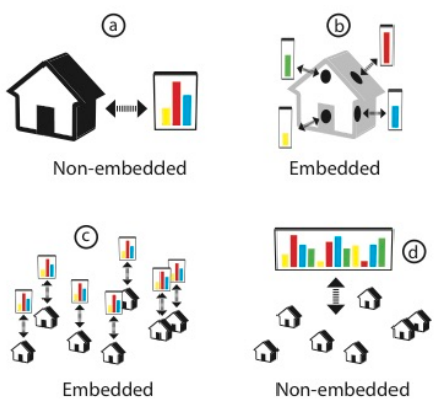
\includegraphics[width=0.5\textwidth]{resources/fundamentals/situated_visualization/embedded_visualization.png}
	\caption{Eingebettete Visualisierung \cite{example_embedded_visualization_concept}}
	\label{img:embedded_visualization}
\end{figure}

\cite[S.~195]{ElSayedNevenA.M.BruceH.ThomasRossT.Smith2015} Eingebettete Visualisierungen (Embedded Visualization) sind situationsbezogene Visualisierungen, welche sehr starken in die physische Umgebung integriert sind. 

Besteht ein Produkt, beispielsweise eine Brille, aus mehreren Einzelteilen, (z. Bsp. Rechter/ Linker Glas, Rahmen, Nasenflügel, Schraube A usw.) und die Daten zu dieser Brille werden neben oder über der Brille visualisiert, gilt die Visualisierung situationsbewusst jedoch nicht als eingebettet.Werden hingegen Teile der Daten welche Einzelteile des physischen Gegenstands betreffen direkt an den Einzelteilen visualisiert, gilt die Visualisierung als eingebettet (embedded).

Abbildung \ref{img:embedded_visualization} zeigt eingebettete und nicht eingebettete (Situated) Visualisierungen. [Kim Marriott et. al Seite 202] zeigen am Beispiel eines Hauses, als physischen Referenten, wie eine Visualisierung die Eigenschaft eingebettet zu sein ändern kann. Wird wie am oberen Beispiel die Daten zu einem Haus in einer Visualisierung am Haus nahe des Hauses visualisiert, gilt die Visualisierung als "Situated" jedoch nicht eingebettet (a). Werden jedoch die Daten welche einzelne Einelemente des Hauses betreffen direkt am betreffenden Einzelelement visualisiert, gilt die Visualisierung als eingebettet (b). Betrachtet man jedoch eine Visualisierung zu mehreren Häusern (z. Bsp. ein Bezirk) und wird aus einer nicht eingebetten Visualisierung wie in a, eine eingebettet Visualisierung wie in (c) abgebildet. 

Eingebettete Visualisierung geht davon aus dass mehrere Teil-Visualisierungen zu jeweiligen physischen Referenten entsprechen. Befinden sich in einem Haus Beispielsweise mehrere Steckdosen und der Stromverbrauch 
für jede Steckdose wird jeweils direkt an jeder Steckdose direkt visualisiert, gilt die Visualisierung als eingebettet. Gibt es in dem Haus jedoch nur eine einige Steckdose, gilt die Visualisierung nicht mehr als
eingebettet.

\vspace{15mm} 
\begin{figure}[H]
	\centering
	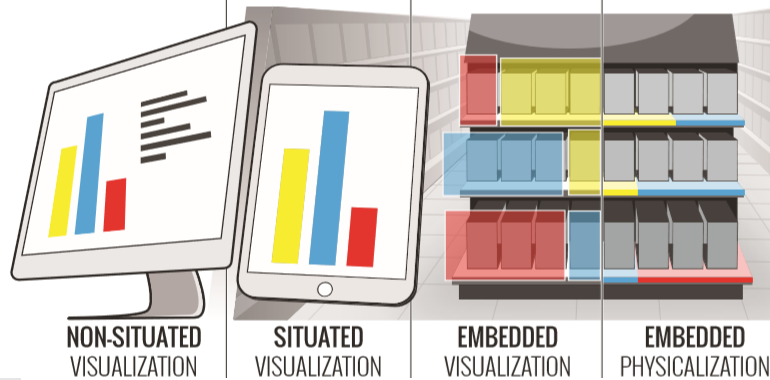
\includegraphics[width=0.5\textwidth]{resources/fundamentals/situated_visualization/Illustration_situated_embedded_visualization.png}
	\caption{Illustration mit unterschiedlichen Visualisierungen am Beispiel von Produkten in einem Supermarkt-Regal \cite{Illustration Visualisierungen}}
	\label{img:Illustration_situated_embedded_visualization}
\end{figure}

Mit Hilfe der Illustration in Abbildung \ref{img:Illustration_situated_embedded_visualization} zeigen \cite{WesleyWillettYvonneJansen} am Beispiel von Produkten welche in einem Supermarkt, in einem Regalen platziert sind, die Eigenschaften von unterschiedlichen Visualisierungen und die damit verbundenen Vor- und Nachteile der jeweiligen Visualisierungsform.\footnote{http://yvonnejansen.me/embedded} Der Vorteil von Non-Situated Visualisierungen (Abbildung \ref{img:Illustration_situated_embedded_visualization} ganz links), ist dass diese flexibler hinsichtlich Standort der Nutzung und Hardwareanforderungen gestaltet werden können. Mit einer Desktop Anwendung kann zum Beispiel die Marktleiterin des Supermarktes Informationen zu sämtlichen Produkten im Markt Visualisieren und ein Überblick erhalten, welche Produkte einen großen Umsatz haben und wie dies über Zeit und Saison variiert. Diese Form der Visualisierung kann je nach dem wo sich die Marktleiterin befindet mehr oder weniger "Situated" sein. Schaut sie sich die Visualisierung zum Beispiel in einem vom Verkaufsraum abgetrennten Büro an, ist sie nicht in der Lage, die im Verkaufsraum platzierten Produkte und die Visualisierung gleichzeitig zu betrachten. Die Visualisierung wäre somit Non-Situated. Möchte sie sich die Beziehung zwischen der phyischen Platzierung der Produkte im Verkaufsraum und deren Umsatz ansehen ist dies nur über abstrakte Beschreibungen oder zum Beispiel mit Hilf einer Karte möglich. Steht sie jedoch im Verkaufsraum und schaut sich die Visualisierung auf einem Tablet an, ist die Visualiseirung Situated (Abbildung \ref{img:Illustration_situated_embedded_visualization} zweite von links)). Auf diese Weise ist es ihr möglich, den Verkaufsraum und die Visualisierung gleichzeitig zu betrachten. Sie kann so eine Beziehung zwischen Verkaufszahl von bestimmten Produkten in Abhängigkeit ihrer Platzierung im Verkaufsraum implizit herstellen.

Auf diese weise ist sie in der Lage, eine Beziehung zwischen der Positionierung der Produkte im Verkaufsraum und den vorhanden Daten in der Visualisierung herzustellen. Die Daten im Kontext zur unmittelbaren Umgebung 
der betreffenden Produkte zu betrachten und vor allem zu überprüfen wird auf diese weise jedoch nicht möglich sein. Wenn zum Beispiel in einem bestimmten Bereich im Verkaufsraum der Umsatz für bestimmte Produkte 
über die vergangen Monate zurück gegangen ist kann Sie einige nicht erfasste Informationen/ Zustände, nicht sehen (Zum Beispiel eine zu schwache Beleuchtung, starker Geruch, Windzug, usw.). Dies wird mit Embedded 
Visualisierung ermöglicht ((Abbildung \ref{img:Illustration_situated_embedded_visualization} dritte von links)).\footnote{(Abbildung \ref{img:Illustration_situated_embedded_visualization} dritte von links) zeigt eine pysikalisierte Visualisierung.}   

%Facsimiles
\cite{WesleyWillettYvonneJansen}Eine Möglichkeit, um Daten im Kontext zu physischen Objekten zu visualisieren, ist auch über die Verwendung von so genannten Faksimiles möglich. Diese sind detailgetreue skalierbare Nachbildungen von Objekten, oder eine Instanz eines Objektes welche durch eine bestimmte Klasse oder Model klar definiert ist. Ein Faksimile wird für gewöhnlich verwendet, falls die Visualisierung am echten physischen Referenten schwierig bis unmöglich ist. Wenn diese zum Beispiel sehr klein (z.Bsp. Atome), sehr groß (z Bsp. ein Flussverlauf) zu Entfernt (z. Bsp: auf einem anderen Planeten) oder sehr fragil bzw. wertvoll sind
(z. Bsp. ein Gemälde). 
In solchen Begebenheiten kann die Nutzung von Faksimiles die räumliche Distanz zum betrachtenden Objekt
reduzieren und es zugänglicher machen. Ein Faksimile kann in manchen Fällen wie der eigentlichen physische Referent betrachtet werden. Vor allem wenn dieser in ausreichender detailgetreue den eigentlichen Referenten nachbildet. Die Nutzung von Faksimiles verringert jedoch oft die Möglichkeit für den Betrachter, den eigentlichen Referenten zu verändern oder wichtige Details zu betrachten. Dies kann durch den Einsatz von Telepräsenz und Teleoperation kompensiert werden.\footnote{Telepräsenz ist eine Form von Videokonferenz und beschreibt die Möglichkeit, virtuell an realen, entfernten Orten Präsent zu sein. Siehe: https://www.itwissen.info/Telepraesenz-telepresence.html [Zuletzt aufgerufen am: 28.06.2018]}

\subsection{(Situated Visualization) - Techniken und Herausforderungen}
Situated Visualization 

%[Schmalstieg und Höllerer] locally situated\ globally situated

% Information seeking mantra von Schneidermann 1996
% Falls die die Informationsmenge zu groß oder zu Komplex wird beschreiben Daniel A. Keim et. al: visual analytics mantra

\begin{table}[htbp]
	\caption{Situatedness vs. Analytic Level}
	\begin{center}
		\begin{tabular}{|l|l|l|}
			\hline
			\textbf{Situatedness}& \textbf{Analytic Level Low} & \textbf{Analytic Level High}\\
			\hline
			\textbf{High } & Situation Awareness & Situated Analytics \\
			\hline
			\textbf{Low} & Information Displays/ Ambient Displays & Visual Analytics/ Traditional Analytics \\
			\hline
		\end{tabular}
	\end{center}
	\label{tab:categorycscw}
\end{table}


%Neven A. M. ElSayed et. all %  Situated Analytics has four primary elements: situated information, abstract information, augmented reality interaction, and analytical interaction

%Herrausforderungen: Unordnung duruch zu viele Daten (Überlagerung). Generell auch bei anderen visualisierungen. Durch limitierter Platz bei AR manchmal besonders verschlimmert. %Registrierungsfehler führen zur falschen platzierung von visualisierungen. 
% Störende\ Ungünstige Visualisierung. Auch wenn Registrierung theoretisch ganz fehlerfrei funtionieren würde, ungünstig sein und die Fähigkeit des Nutzers wichtige Informationen von nicht relevanten Informationen. 

% In folgendem werden Techniken für die Bewältigung dieser Herrausforderungen vorgestellt. 

Data Overlay 

% la

% Labeling und Annotationen


\section{Computerunterstützte Kollaboration}

Durch die Verwendung des zu entwickelnden Systems, sollen zum einen Anwendungsszenarien unterstützt werden, in welchen Nutzer, 
Rückmeldungen zur Gestaltung von Produkten kommunizieren können, zum anderen soll anderen Nutzern 
ermöglicht werden diese Rückmeldungen zu explorieren. Diese Kommunikation soll eine Kollaboration von 
mehreren Nutzern, mit dem Produkt im Mittelpunkt zu ermöglichen, 
und zum Ziel haben, die Qualität der Produkte und die damit Verbunde Kundenzufriedenheit zu verbessern.     

In der computerunterstützten, kooperativen Zusammenarbeit (en. Computer-Supported Cooperative Work (CSCW)) 
ist eine Kategorisierung die Tom Rodden \cite[S.~2]{Rodden1992} beschreibt, sehr verbreitet.  

Rodden betrachtet bei dieser Kategorisierung zwei Dimensionen in der Kommunikation zwischen Nutzern. 
Die räumliche Distanz zwischen den Nutzern und die zeitliche Differenz im Nachrichtenaustausch, und macht eine 
Unterteilung in Remote oder Co-Located und Synchron oder Asynchrone Kommunikation.

Betrachtet man die zeitliche Dimension, können mehrere Nutzer zur gleichen Zeit (synchron) miteinander kommunizierender 
oder zu unterschiedlichen, also (asynchron/ zeitlich unabhängig voneinander) kommunizieren. Die räumliche Dimension 
gibt Aussage darüber ob sich die Nutzer während der Kommunikation am gleichen Ort befinden (Co-located) oder entfernt voneinander sind (Remote). 

\cite[S.~188]{ElSayedNevenA.M.BruceH.ThomasRossT.Smith2015} beschreiben eine weitere Form, welche eine Mischform von Remote und Co-located bildet. 
Bei dieser Form von Kollaboration können eine Teilmenge der Nutzer sich am gleichen Ort befinden, während ein anderer Teil, entfernt, 
also (Remote) mittels Telepräsenz an der Kommunikation teilnehmen. 

Schmalstieg und Höllerer \cite{DieterSchmalstieg2016} beschreiben auf Grundlage dieser Unterteilung, mögliche 
Anwendungsgebiete für AR Systeme (Siehe Tabelle \ref{tab:categorycscw}).

\cite{DieterSchmalstieg2016} In Co-Located und synchronen Anwendungsszenarien (z. Bsp. eine Besprechung in einem Besprechungsraum), können 
Augmented Reality Anwendungen, die Nutzern dabei unterstützen, Informationen im gemeinsamen Raum zu betrachten zu manipulieren und zu diskutieren. 

In Remote und synchronen Szenarien können AR Systeme es ermöglichen dass ein Teilnehmer (Nutzer 1), einem anderen Teilnehmer (Nutzer 2) an einem entfernten Ort, Informationen über dessen reale Umgebung zu zeigen 
kann (zum Beispiel eine Installations- oder Reparatur-Anleitung), ohne dass der zweite Teilnehmer (Nutzer 2) seine Aufmerksamkeit von seiner realen Umgebung abwenden muss.

\begin{table}[htbp]
\caption{Kategorisierung Computer unterstützter Kooperationssysteme in Bezug zu AR}
	\begin{center}
		\begin{tabular}{|l|ll|}
		\hline
		 & \textbf{Co-located} & \textbf{Remote}\\
		\hline
		\textbf{Synchronous} &  AR shared space & AR telepresence \\
		\textbf{Asynchronus} & AR annotating/ browsing (in-situ) & Generic sharing\\
		\hline
		\end{tabular}
	\end{center}
	\label{tab:categorycscw}
\end{table}

\cite[S.~362]{DieterSchmalstieg2016} Asynchrone Szenarien sind bisher in AR weniger verbreitet. Der wichtigste Anwendungsfall nach Schmalstieg und Höllerer, 
ist das Erstellen von Annotationen auf der physischen Umgebung und das spätere Durchforsten und Editieren, dieser Annotationen durch andere Nutzer. 
%You might think of this application as a sort of virtual graffiti.

Rodden \cite{Rodden1992} beschreibt dass verteilte, asynchrone Kollaboration, es ermöglicht, Inhalte von unterschiedlichen Nutzern zu unterschiedlichen Zeiten, zu erfassen und.
Dies biete einige Vorteile.

- Erzeugung von viel breitere Gruppendiskussionen und Aufzeichnung dieser Diskussionen(Report) (z.Bsp. Foren, Community Beiträge).\cite{Rodden1992} cite{Benbunan-Fichet} 
- Gibt Nutzern die Flexibilität, immer dann Beiträge zu erstellen wenn diese Zeit dazu haben.
- Ermöglicht, Nutzern sich mit Teilproblemen befassen für das sie sich am besten befähigt fühlen.
- Zusammensetzung von Informationen aus eine Vielzahl von Quellen und Nutzern


Roden \cite{Rodden1992} ordnet asynchrone Kollaboration zu den Co-Authoring Systemen. Diese sind Systeme, welche mehreren Nutzern, asynchrone Zusammenarbeit 
an einem Artefakt ermöglichen. Jeder Nutzer kann dabei an einem Teil des Dokumentes arbeiten und die Ergebnisse werden zusammengeführt. Asynchrone Kollaboration 
unterstützt laut Rodden einen Grundlegenden Teil von Kooperation, indem es die 
% can produce broader discussions and more complete reports from group discussions than their face-to-face counterparts
% enabling people to contribute whenever they have time to provide input
% they can work on the part of the problem that they feel most qualified to address
% can combine information from a variety of sources

% Co-authoring systems aim to support some of the most fundamental parts of cooperation by supporting the negotiation processes
% for commenting - multiple users working on 
% store and forward and real-time communication systems

%notwendigkeit für unterscheidung zwischen private, public oder direkte nachrichten 

%[Rodden seite 20]
% [Rodden seite 24] Co-authoring systems aim to support some of the most fundamental parts of cooperation by supporting the negotiation processes % for commenting %multiple users working on % [Rodden seite 24]store and forward and real-time communication systems. %
%The general model adopted by these systems is that of asynchronous co-operation with each user working independently on a portion of the document. Reviews and comments are added to the document by annotating sections of the document. 

\section{Usability}

% Ziel der Arbeit ist ein Weg zu finden um effektiv und effizient Produktdesignbeschreibungen an Produkten zu zeigen mit einsatz von Augmented Realiy und verschiedene Techniken zu 
%vergleichen. Dafür muss ein besonderer Fokus auf die Usablity gelegt werden. Daher hier usability...
Einen besonderen Fokus legt diese Arbeit auf die Usability des zu konzipierenden Systems. Daher wird in folgendem Abschnitt die Begriffsdefinition von Usablity näher beleuchtet, es werden einige 
gängige Methoden für die nutzenorientierte Gestaltung und Entwicklung von Systemen vorgestellt und abschließend Methoden für Usability Tests und Evaluierung erläutert. 

\subsection{(Usability) - Definition} \label{UsaDef}

% Begiffserklärung von Usability
In der Norm-reihe ISO 9241 welches als ein internationaler Standard, Richtlinien für die Gestaltung von Mensch-Computer-Interaktionen beschreibt, wird im ISO Norm 9241-11,  Usability wie folgt definiert:
``das Ausmaß, in dem ein Produkt durch bestimmte Benutzer in einem bestimmten Nutzungskontext genutzt werden kann um bestimmte Ziele effektiv, effizient und zufriedenstellend zu erreichen.``

% Usablity nicht nur Gestaltung der Nutzeroberfläche
\cite{MichaelRichter2016; MaryBethRossonJohnM.CarrollDianeD.Cerra2002} Usablity wird  oft als ein Qualitätskriterium für die Gestaltung der Benutzerschnittstelle verstanden. Dies ist jedoch nicht ganz richtig.

%Die Benutzbarkeit eines Systems muss im Kontext seiner Verwendung beurteilt werden.[Michael Richter, Markus Flückiger]
Dass die Usability eines Systems nach dessen Nutzungskontext zu beurteilen ist verdeutlichen \cite{MichaelRichter2016} an einem konkreten Beispiel für die Erfassung 
von Kurznachrichten (SMS) mit dem Aufkommen von Mobiltelefonen.  Bevor Smartphones mit Touch-Displays verbreitet waren, hatten Mobiltelefone oft rein numerische Tastaturen sodass, das Erfassen 
von Textnachrichten über die Nutzung der numerischen Tasten erfolgen musste. Indem zum Beispiel in kurzen Zeitabständen zwei mal auf die Taste "2" gedrückt wurde, wurde zu Beispiel der Buchstabe 
``B" eingegeben. Diese Eingabemethode wurde oftmals von vielen Nutzern als umständlich empfunden. Jedoch konnte auf diese Weise effizient und zufriedenstellend die Aufgabe, eine Kurznachricht 
zu erfassen erfüllt werden. Zudem war diese Methode einfach zu erlernen und einprägsam. Somit wies dieser Ansatz für den damaligen Stand der Technik eine hohe Usablity auf. 

% Usablity nicht nur User friendly
\cite{Nielsen1994,RexHartson2012} Oft wird Usablity auf die Eigenschaft eines Systems reduziert besonders benutzerfreundlich (en. User- friendly) zu sein. Der Begriff Usabliy umfasst jedoch mehr Aspekte. 

\cite{Nielsen1994} Mit dem Begriff "User- friendly" als Synonym für Usablity, würde impliziert werden dass die Bedürfnisse von Benutzern mit nur einer Dimension eines Systems beschrieben werden könne. 
In der Realität haben jedoch unterschiedliche Nutzer, verschiedenartige Bedürfnisse. Ein System welches zu einem Benutzer freundlich erscheint, könnte unter Umständen von einem anderen Nutzer als 
lästig empfunden werden.

% Eine Teilmenge der Systemazeptanz 
Nielsen \cite{Nielsen1994} Unterteilt Akzeptanzkriterien für ein Systems in soziale und praktische Kriterien.

Soziale bzw. ethische Akzeptanzkriterien sind solche, welche die Nutzer von der Nutzung eines Systems abhalten, auch wenn praktische Akzeptanzkriterien sehr gut erfüllt werden. 

Spiekermann führt in \cite[S.~285]{Spiekermann2016} interessante Beispiele für soziale Akzeptanzkriterien für IT Systeme und stellt Methoden vor wie bei der Gestaltung von IT Systemen 
soziale bzw. ethische Kriterien berücksichtigt werden können.\footnote{\cite[S.~285]{Spiekermann2016} Sie beschreibt am Beispiel eines Körperscanners an Flughäfen, dass trotzt  
Berücksichtigung vieler praktischer Aspekte wie Ergonomie, effizienter und effektiver Aufgabenerfüllung ein solches System wenig Akzeptanz von den Nutzern finden kann. 
Beispielsweise fühlten sich Passagiere unangenehm wenn, der Bildschirm auf welchem die nackten Umrisse ihrer Körper zu sehen war, so platziert wurde, dass andere Passagiere ihren Körper sehen konnten.
Umstellung von Nackt- Körperscannern auf alternative System wegen fehlender Nutzerakzeptanz: https://www.wired.com/2013/01/tsa-abandons-nude-scanners/ [Zuletzt aufgerufen am: 26.06.2019]}

Um die gewünschte Funktionalität zu ermöglichen, wird mit Augmented Reality Anwendungen viel Informationen über die Umgebung des Nutzers erhoben.\cite[S.~3]{Roesner2013} Es wird auf die Kamera und gegebenenfalls 
auf den Lautsprecher und verschieden Sensoren (Gyroskop, Accelerometer usw.) dauerhaft zugegriffen. Dies birgt Risiken dass diese Daten missbräuchlich genutzt, gestohlen und die Privatspähehe von Nutzern verletzt 
werden kann. \cite[S.~9]{Templeman2012} In einer Studie konnte Beispielsweise bewiesen werden, dass mit Kamera und Sensordaten eines Smartphones die Umgebung des Nutzers detailliert genug
rekonstruiert werden kann, um sensible Kontodaten auf einem Kontoauszug ablesen zu können. \cite{Roesner2013,Lebeck2018} stellen weitere Risiken für die Beeinträchtigung der Privatsphäre von Nutzern vor welche als 
soziale Akzeptanzkriterien bei der Gestaltung von Augmentend Reality Systemen beachtete werden sollten. 

%TODO relavant für diese Arbeit könnte die Verwendung von Sensor und Videodaten sein. Verweis auf Privacy in Mixed Reality Studien.

Als praktische Kriterien führt er Eigenschafen wie Kosten, Kompatibilität, Zuverlässigkeit sowie Nutzbarkeit auf. Die Eigenschaft Benutzbarkeit teilt er in die Eigenschaften Nützlichkeit (en. Utility) und Gebrauchstauglichkeit (en. Usability) auf. Unter Utility ist zu verstehen ob ein System mit den Funktionalitäten die es bereitstellt prinzipiell in der Lage ist, die Aufgabe zu erfüllen wozu sie konzipiert wurden.

Die Eigenschaft Geruchstauglichkeit gliedert er in folgende fünf Teileigenschaften: 

\begin{itemize}
	\item Einfach zu erlernen.
	\item Effizient in der Nutzung.
	\item Leicht zu merken. (Ein Nutzer welcher das System einmal verwendet hat, sollte in der Lage sein nach einer längeren Pause das System zu nutzen ohne es erneut erlernen zu müssen.)
	\item Wenig Fehler. (Das System sollte zu möglichst wenig Fehler während der Nutzung führen. Im Falle das Fehler auftritt, sollte es möglich sein dass sich das Systems von diesem Fehler erholt und die Nutzung fortgeführt werden kann.)
	\item Subjektive Zufriedenstellung (Das System sollte angenehm zu nutzen sein. So dass Nutzer auch subjektiv zufriedengestellt werden während sie das System nutzen.)
\end{itemize}

%7 Kritärien nach ISO 9241 Teil 110 - ASSEFIL) 
Im ISO Norm  9241-110 sind diese Kriterien, als Grundsätze zur Dialoggestaltung wie folgt aufgeführt:

\begin{itemize}
	\item Aufgabenangemessenheit \footnote{Beispiele für Aufgabenangemessenheit ab Seite 5: https://www.medien.ifi.lmu.de/lehre/ss16/id/ISO\_9241-10.pdf [zuletzt aufgerufen am: 26.06.2019]}
	\item Selbstbeschreibungsfähigkeit
	\item Steuerbarkeit
	\item Erwartungskonformität
	\item Fehlertoleranz
	\item Individualisierbarkeit
	\item Lernförderlichkeit
\end{itemize}


%TODO: Folgerung für diese Arbeit!!!

\subsection{Usablity Engineering}

\cite{MichaelRichter2016} Im laufe der Zeit haben sich verschiedene Fachrichtungen (wie z. Bsp: Human Computer Interaction (HCI), Human Factors, Interaction Design, Usability Engineering, 
User centered Design (UCD), User Experience (UX) und Design Thinking)  entwickelt welche nutzenorientierte Methoden für die Entwicklung von Technologien und neuen Anwendungen verfolgen. 

% Usablity Engineering
\cite{MaryBethRossonJohnM.CarrollDianeD.Cerra2002} Als eines dieser Fachrichtungen wurde die Fachrichtung Usablity Engineering von Usability Fachleuten bei Equipment Corparation ins Leben gerufen.  
Der Begriff Usability Engineering steht für die Konzeption und Techniken für die Planung, Verifizierung und Abdeckung von Usability Zielen eines Systems. Das Ziel von Usability Enginieering ist, 
messbare Usability Ziele in den frühen Phasen des Softwareentwicklungsprozesses zu definieren und einen Rahmen zu schaffen diese Ziele im laufe der Entwicklung stetig überprüfen zu können 
um sicherstellen zu können dass diese erreicht werden.

Nielsen beschreibt in \cite{Nielsen1994} folgende Phasen im Lebenszyklus von Projekten mit Software Engenieering Methoden.

\vspace{10mm}
\textbf{Analyse der Nutzer / Aufgaben und Ziele}  
 
In dieser Phase der Usability Engineering werden alle Nutzer identifiziert, die mit dem System in Berührung kommen werden. Als Nutzer sollten alle Personen verstanden werden welche mit dem 
System oder mit Artefakten des Systems in Berührung kommen werden. Dies können Personen beinhalten welche das System installieren, konfigurieren, warten, administrieren aber auch Endkunden oder 
Personen die das System selbst nie sehen werden jedoch Ergebnisse von dem System erhalten werden. In einigen Fällen, ist es einfacher potenzielle Nutzer von einem System zu identifizieren und deren 
Charakteristiken zu studieren. Zum Beispiel für Produkte die in einer bestimmten Abteilung eines bestimmten Unternehmens eingesetzt werden sollen. Schwieriger ist es hingegen für Produkte 
welche von einer breiteren Menge von Nutzern genutzt werden soll. Es sollten Eigenschaften von Nutzern studiert werden welche für das Nutzen des Systems relevant sein könnten wie zum Bsp. 
Wieviel Erfahrung  hat der Nutzer in Verwendung von solchen Systemen und Endgeräten, Bildungsstand, Alter. etc. Dieser Schritt ist wichtig um die Lernfähigkeit von Nutzern besser einschätzen zu 
können und so Kriterien für die Komplexität der Nutzeroberfläche zu bestimmen.
%TODO Beispiel von Buch Verkauf MichalelRichter

% task analysis
Sobald die Nutzer identifiziert und deren Eigenschaften und Bedürfnisse analysiert wurden, werden die Ziele und Aufgaben der Nutzer analysiert. Wie bewältigen die Nutzer aktuell Aufgaben um 
ihre Ziele zu erreichen? Hierbei sollte beobachtet werden welche Informationen die Nutzer benötigen, welche Ausnahme oder Not Situationen  auftreten und wie die Nutzer in diesen Situationen handeln. 
Es sollte beobachtet werden ob die Nutzer das aktuell verwendete System in irgendeiner weise umgehen (en. Workarounds anwenden). Zudem sollten die im Bezug auf die zu lösende Aufgabe, verwendeten 
Terminologien notiert werden. Diese können später als eine Quelle für Metapher bei der Gestaltung der neun Nutzeroberfläche verwendet werden. 

% functional analysis
Im nächsten Schritt werden die benötigten Funktionalitäten des neuen Systems analysiert und Möglichkeiten erforscht wie diese mit dem neuen System erzielt werden können. 
Es ist wichtig dass in diesem Schritt die Mögliche Umsetzung der Funktionalitäten sich nicht ausschließlich an Lösungen von bereits bestehenden Systemen orientiert sondern 
bessere geeignete Umsetzungsmöglichkeiten erkundet werden.

% evolution of the user
Zuletzt werden in dieser Phase Möglichkeiten erforscht wie sich das Nutzungsverhalten der Nutzer in Zukunft mit der Nutzung des neuen Systems entwickeln könnte. Dieser Schritt wird  
benötigt um das neue System flexibel genug und offen für neue Anforderungen  gestalten zu können welche in der Zukunft auftreten könnten. %TODO Mach hier noch ein Beispiel! 

\vspace{10mm}
\textbf{Analyse bestehender Produkte} 
 
In dieser Phase werden bestehende Produkte analysiert. Diese können für die Konzeption des neuen Systems als Prototypen dienen. Da bestehende Systeme vollständig 
umgesetzte Funktionalitäten beinhalten, können diese einfach getestet werden.    
Diese Systeme können heuristisch evaluiert werden, es können Nutzer Studien durchgeführt werden oder es kann eine vergleichende Analyse durchgeführt werden falls mehrere Systeme zur 
Verfügung stehen. Auf Basis der Informationen die, in der Phase "Kenne deiner Nutzer" zusammengetragen wurden, wird in dieser Phase analysiert wie gut die  Funktionalitäten und Interaktionstechniken 
bestehender Systeme die Nutzer bei der Umsetzung ihrer Aufgaben unterstützen. Das Lesen von technischen Produktrezessionen kann in dieser Phase auch hilfreiche Informationen über bestehende Systeme geben. 

\vspace{10mm} 
\textbf{Usablity Ziele definieren} 

Wie im Abschnitt \ref{UsaDef} beschrieben, setzt sich die Usability eines Systems nicht nur aus einer Eigenschaft zusammen sondern gliedert sich in mehrerer Eigenschaften wie Erlernbarkeit, Fehlertoleranz etc. auf. 
Oft ist es nicht möglich alle Usablity Kriterien mit gleicher Gewichtung zu priorisieren. In dieser Phase werden auf Grundlage der Analyse von Nutzern und deren Aufgaben und Zielen, Prioritäten für Usability Kriterien definiert. 

Dafür werden die Usablity Kritärien operationalisiert und in messbaren Zielen ausgedrückt. Meistens werden Messintervalle für angestrebte Werte, für minimal zu erreichende Werte und theoretisch optimale Werte definiert. 
Als minimal zu erreichende Werte sind, gelten der Regel Werte welche aktuell mit dem System erreicht werden kann. Usability Ziele für neue Versionen von bestehenden Systemen oder für Systeme für welche vergleichbare andere 
Systeme existieren, festzulegen ist deutlich einfacher als für neue Systeme wozu keine Vergleichswerte vorliegen. Ein Vorgehen für solche Systeme ist, einige mit dem System zu lösende Aufgaben zu definieren und mehrere Usablity Spezialisten nach realistischen Werten zu fragen welche erzielt werden könnten.

\vspace{10mm} 
\textbf{Prototypen}

% Vertikale/ Horizontale

%Warum? Vorteile?

% Prototyping für 3D oberflächen?

% Noch weitere aber hier nur kurz. 

\subsection{Personas, Szenarien und Use Cases}

% Personas

% Szenarios

% Use Cases

\subsection{Usablity Tests und Evaluirung}

\section{Produktbewertungen}


